\subsection{Serveer de web-app via Flask}
Om te voorkomen om nog een applicatie zoals Nginx of Apache op de Raspberry pi te moeten installeren, configureren en draaien voor het serveren van de web-applicatie, leek het ons een goed idee om deze via Flask bereikbaar te maken. Dit wat helemaal niet lastig en hebben we op een vrij simpel maar toch elegante manier opgelost. Als de route \quotes{/} wordt aangevraagd, zal de index.html worden teruggegeven. Als er iets anders wordt opgevraagd, zal er worden gekeken of dit bestand bestaat op de Raspberry Pi. Als dit niet het geval is zal de webserver een 404 error terug geven. In figuur \ref{fig:frontend} is de code te zien.\\ 

\subsection{Op de gedetecteerde ballen afrijden}
Voor het afrijden op de bal hebben we een extra klasse gemaakt die gebruik maakt van de object detectie klasse de \quotes{detector}. Met behulp van een callback die de detectie terugkrijgt kunnen er acties worden ondernomen op basis van de positie van de bal. Allereerst leek het ons een goed idee om met een PID-controller op de bal af te rijden en bij te sturen waar dit nodig was. Echter ging de PID-controller een beetje gek doen op verschillende afstanden tot de bal. Als de Robot redelijk dichtbij was en werd aan gezet, zorgde de PID-controller er voor dat de robot een zwaai naar links deed en het doelwit ver voorbij ging. De robot was dan de detectie kwijt of vond een andere tennisbal. Om de PID-controller accurater te krijgen hebben we geprobeerd de PID waardes aan te passen en zo de controller wat bij te stellen. Dit duurde erg lang omdat de robot steeds verplaatst moest worden om dit opnieuw te kunnen testen. Omdat we -- Joey en Sergi -- niet dicht bij elkaar zijn, maakt dit het wel erg lastig en tijdrovend. We zijn van mening dat we dit op school veel beter hadden kunnen bijstellen. Echter moesten we nu met een simpele en snelle oplossing komen. Daarom zijn we richting een formule gedaan die aan de hand van delta's de snelheid van de motoren aanpast. De robot komt hierdoor altijd wel goed uit, ook al is het misschien wat langzamer. De code die er voor zorgt dat de robot naar de bal rijd is te zien in figuur \ref{fig:callback}.\\

In de code is te zien dat de PID-controller er nog wel in zit. En optioneel gebruikt kan worden. Dit kan worden gedaan door de \quotes{detector} klasse aan te maken met een True argument.\\

\begin{figure}[H]
    \centering
    \begin{minted}{python}
    @app.route('/', defaults={'path': ''})
    @app.route('/<path:path>')
    def serve(path):
        if not path:
            path = "index.html"
    
        if path_to_file_exists(path):
            return send_from_directory(app.static_folder, path)
        else:
            return abort(404)
            
    def path_to_file_exists(path):
        if not path:
            return False
            
        full_path = app.static_folder + "/" + path
        
        return os.path.exists(full_path)
    \end{minted}
    \caption{Flask code voor het serveren van de frontend applicatie.}
    \label{fig:frontend}
\end{figure}

\begin{figure}[H]
    \centering
    \begin{minted}{python}
    def callback(self, detections):
        detection = self.get_nearest_detection(detections)
        
        if self.collected(detection):
            self.done()
            return
        
        direction, distance = self.get_control(detection)
        left, right = self.get_speed(direction, distance)
        
        self.zumo.run('left', left)
        self.zumo.run('right', right)
    
    @staticmethod
    def get_nearest_detection(detections):
        detection = max(detections, key=lambda d: d.width)
        return detection
    
    def collected(self, detection):
        return detection.width > self.CLOSE_POINT
    
    def done(self):
        self.zumo.run('stop')
        self.pause()
        print("Collected ball")
    
    def get_control(self, detection):
        if self.use_pid:
            direction_control = 
                self.direction_pid(detection.position)
            distance_control = 
                self.distance_pid(detection.width)
        else:
            direction_control = detection.position - 0.5
            distance_control = 1 - detection.width
        return direction_control, distance_control
    
    def get_speed(self, direction, distance):
        speed = abs(max(distance * self.MAX_SPEED, 150))
        left = abs(self.MIDDLE_POINT - direction) * speed
        right = abs(self.MIDDLE_POINT + direction) * speed
        return left, right
    \end{minted}
    \caption{De callback functie die acties onderneemd aan de hand van de detectie.}
    \label{fig:callback}
\end{figure}

\subsection{Ballen naar het verzamelpunt brengen}
Om de ballen naar het verzamelpunt te brengen maakte we gebruik van meerdere services. Eentje daarvan was de positie service door middel van BLE. De redenen dat we deze service nodig hadden was zodat we een start positie konden definiëren, de auto een stukje laten rijden en daarna een eind positie berekenen.\\
\begin{figure}[H]
    \centering
    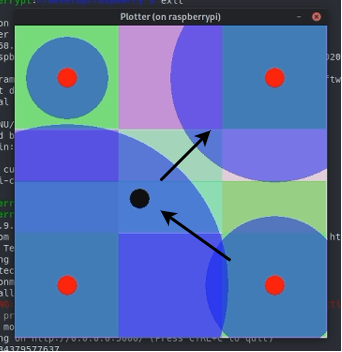
\includegraphics[width=200pt]{img/plotter_angle.png}
    \caption{Pijlen met de berekende route}
    \label{fig:plotter_angle}
\end{figure}

Nu we beide posities weten kunnen we gemakkelijk de hoek berekenen waar de robot naartoe rijdt. Dit kunnen we doen door eerst de hoek te berekenen van de eindpositie naar het verzamelpunt, en dan het verschil tussen beide hoeken te draaien. Daarna hoeven we alleen nog maar rechtdoor te rijden en te controleren of we dichtbij het verzamelpunt zijn door middel van de positie service.\\

Het enigste probleem waar we vaak tegen aanliepen was dat de kabels een grote invloed hadden in hoe recht de robot reedt. Hierdoor gebeurde het vaak dat de robot lichtelijk afdwaalt naar links of naar rechts en daardoor de berekening niet meer klopt.\\

\subsection{Logica voor het verzamelpunt, zones en modus maken}
Het kiezen van een verzamelpunt en zones kan worden gedaan door middel van de web app. De instellingen worden door de flask-server ingesteld en door de \quotes{Zones} klasse uitgelezen. Deze instellingen worden later gebruikt tijdens het berekenen van de route die de robot moet rijden naar een verzamelpunt of zone.\\

Nadat de robot een bal heeft verzameld moet de robot terug rijden naar de geselecteerde zone. Dit gebeurt door middel van de laatste bekende hoek van het terug brengen van de bal. Door deze hoek te combineren met de huidige positie en de positie van de zone kunnen we een nieuwe hoek berekenen waarnaar de robot naartoe moeten draaien. Vervolgens hoeven we alleen maar rechtdoor te rijden om bij onze eindbestemming uit te moeten komen.

\subsection{Navigatie klasse maken}
De navigatie klassen is een state-pattern die er voor zorgt dat al de hierboven genoemde technieken combineert in één systeem. De robot begint als eerste met het zoeken van een tennisbal door middel van object detectie. Vervolgens brengt de robot deze bal naar het geselecteerde verzamelpunt. Daarna reed de robot terug naar de geselecteerde zone. Vervolgens begon het hele traject weer opnieuw.

\begin{figure}[H]
    \centering
    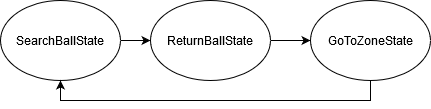
\includegraphics[width=200pt]{img/state_pattern.png}
    \caption{De mogelijke state transitions}
    \label{fig:state_pattern}
\end{figure}

\subsection{Binnen de zones blijven}
De binnen de zones blijven is een beetje van scope verandert. Dit kwam omdat het erg warrig gedefinieerd stond in het onderzoek. De uiteindelijke versie heeft voornamelijk de taak gekregen om naar de juiste zone te rijden en daar te gaan zoeken naar tennis ballen.

% Is niet af gekomen. Ander hoofdstuk?
\subsection{Obstakels ontwijken}
Deze feature is er helaas niet in gekomen, dit komt voornamelijk omdat we geen tijd hadden om deze nice-to-have feature te implementeren. Verder namen we aan dat er niet echt  obstakels op een tennisbaan zouden staan. Dus dit leek het ons niet een heel groot probleem om deze feature weg te laten.
